% Task 4 — Regional Node Candidates
% Northeast Megaregion Freight Network Design
% All floor-area figures in square feet (sf) unless otherwise noted.

\section{Task 4 — Regional Hub Candidate Screening}

Task 4 builds the pre-screened pool of regional hub candidates that feeds the set-cover
optimization in Task 5. The input is a raw CoStar commercial real-estate pull covering all
14 Northeast states; the output is a curated list of logistics facilities that satisfy the
minimum capacity, operational status, and facility-type requirements for serving as a
regional distribution hub.

\subsection{Data Source and Raw Pool}

CoStar property records were obtained for all 14 NE states, yielding \textbf{2,064
facilities} after initial aggregation. Every record includes rentable building area (RBA),
available floor space, building class, secondary use type, geographic coordinates,
number of loading docks, and building status. All 2,064 records are classified as
logistics-related (Warehouse or Distribution) by construction of the CoStar query, so no
type-based pre-filter is necessary at the raw stage.

\subsection{Screening Filters}

Three sequential filters reduce the raw pool to the final primary candidate set:

\paragraph{Filter 1 — Operational status.}
Facilities are classified into three availability categories based on building status:
\textit{direct existing} (2,040 properties), \textit{pipeline / under construction} (22),
and \textit{proxy / final planning} (2). Only \textit{direct existing} facilities are
eligible as primary candidates; pipeline and proxy properties represent locations whose
physical plant does not yet exist or is not yet verified, making them unsuitable for
near-term hub activation under the 2025/2030 planning horizon.

\paragraph{Filter 2 — Minimum capacity threshold.}
Of the 2,040 direct existing facilities, \textbf{1,885} meet the minimum rentable building
area of 200{,}000~sf. This threshold corresponds to the lower bound on regional hub
capacity derived from the paper's sizing analysis: a facility must be large enough to
consolidate and cross-dock truck freight at the regional scale. Facilities below this
floor area are retained in the broader pool
(\texttt{preprocessed\_capacity\_location.csv}) as a fallback for sparse regions but are
excluded from the primary candidate list.

\paragraph{Filter 3 — Available space floor.}
The primary candidate criterion further requires that
\texttt{usable\_available\_space\_sf} $\geq$ 200{,}000~sf, ensuring that the recorded
available-space figure, not merely the total building footprint, meets the hub sizing
requirement. After applying all three filters, \textbf{1,862 primary regional hub
candidates} remain.

\subsection{Candidate Pool Characterization}

Table~\ref{tab:task4-pool} summarizes the primary candidate pool.

\begin{table}[H]
  \centering
  \caption{Primary regional hub candidate pool summary (1,862 facilities).}
  \label{tab:task4-pool}
  \begin{tabular}{lrr}
    \toprule
    Metric & Value \\
    \midrule
    Total candidates & 1{,}862 \\
    Warehouse & 1{,}243\,(66.8\%) \\
    Distribution centre & \phantom{0}619\,(33.2\%) \\
    Class A & \phantom{0}624\,(33.5\%) \\
    Class B & \phantom{0}758\,(40.7\%) \\
    Class C & \phantom{0}476\,(25.6\%) \\
    Median usable available space & 304{,}224~sf \\
    Mean usable available space & 316{,}005~sf \\
    Min / max usable available space & 200{,}000 / 500{,}000~sf \\
    Total usable available capacity & 588.4~M~sf \\
    Median number of loading docks & 27 \\
    Median year built & 1987 \\
    Regions covered ($\geq$1 candidate) & 50 of 50 \\
    \bottomrule
  \end{tabular}
\end{table}

The pool is composed of two facility sub-types: warehouses (67\%) and distribution
centres (33\%). Distribution centres carry a higher median RBA (310{,}323~sf vs.\
283{,}089~sf for warehouses), reflecting their design for active cross-docking rather
than storage. Building class is roughly split between A (34\%) and B (41\%), with Class
C representing legacy stock (26\%); all three classes are retained because the MIP in
Task 5 selects on geographic coverage and capacity rather than on facility quality.

\subsection{Geographic Distribution}

Table~\ref{tab:task4-state} reports the candidate count and total usable capacity by
state.

\begin{table}[H]
  \centering
  \caption{Primary candidates and total usable capacity by state.}
  \label{tab:task4-state}
  \begin{tabularx}{\textwidth}{lrrr}
    \toprule
    State & Candidates & Total usable capacity (Msf) & Median RBA (sf) \\
    \midrule
    PA & 456 & 154.6 & 320{,}470 \\
    NY & 313 & \phantom{0}92.2 & 267{,}442 \\
    VA & 236 & \phantom{0}73.7 & 291{,}041 \\
    NJ & 231 & \phantom{0}87.9 & 362{,}019 \\
    MA & 196 & \phantom{0}58.3 & 273{,}660 \\
    MD & 191 & \phantom{0}56.3 & 267{,}959 \\
    CT & \phantom{0}94 & \phantom{0}28.1 & 272{,}051 \\
    WV & \phantom{0}30 & \phantom{0}18.0 & 169{,}094 \\
    DE & \phantom{0}39 & \phantom{0}11.8 & 250{,}000 \\
    NH & \phantom{0}27 & \phantom{0}\phantom{0}8.3 & 277{,}192 \\
    RI & \phantom{0}23 & \phantom{0}13.8 & 150{,}351 \\
    ME & \phantom{0}18 & \phantom{0}10.3 & 144{,}071 \\
    VT & \phantom{0}\phantom{0}5 & \phantom{0}\phantom{0}4.4 & 143{,}794 \\
    DC & \phantom{0}\phantom{0}3 & \phantom{0}\phantom{0}1.9 & 139{,}612 \\
    \bottomrule
  \end{tabularx}
\end{table}

Pennsylvania dominates the pool with 456 candidates (24.5\%) and 154.6~Msf of usable
capacity, reflecting its role as the primary inland logistics corridor in the Northeast.
New Jersey ranks second in density (231 candidates, median RBA 362{,}019~sf), consistent
with its position as the highest-throughput single-state logistics market in the region.
The smallest state pools --- Vermont (5), DC (3), and Rhode Island (23) --- present a
potential coverage risk for hub selection; the Task 5 MIP addresses this by allowing a
wider geographic assignment radius and using the broader
\texttt{preprocessed\_capacity\_location.csv} pool as a fallback for sparse regions.

Every one of the 50 Task~3 regions contains at least 7 primary candidates, with a
mean of 37.2 candidates per region and a maximum of 121 candidates in the most
logistics-dense region. This density provides the Task~5 MIP with a rich feasible set
for each coverage decision.

Figure~\ref{fig:task4-map} plots the geographic distribution of all primary candidates
across the megaregion.

\begin{figure}[H]
  \centering
  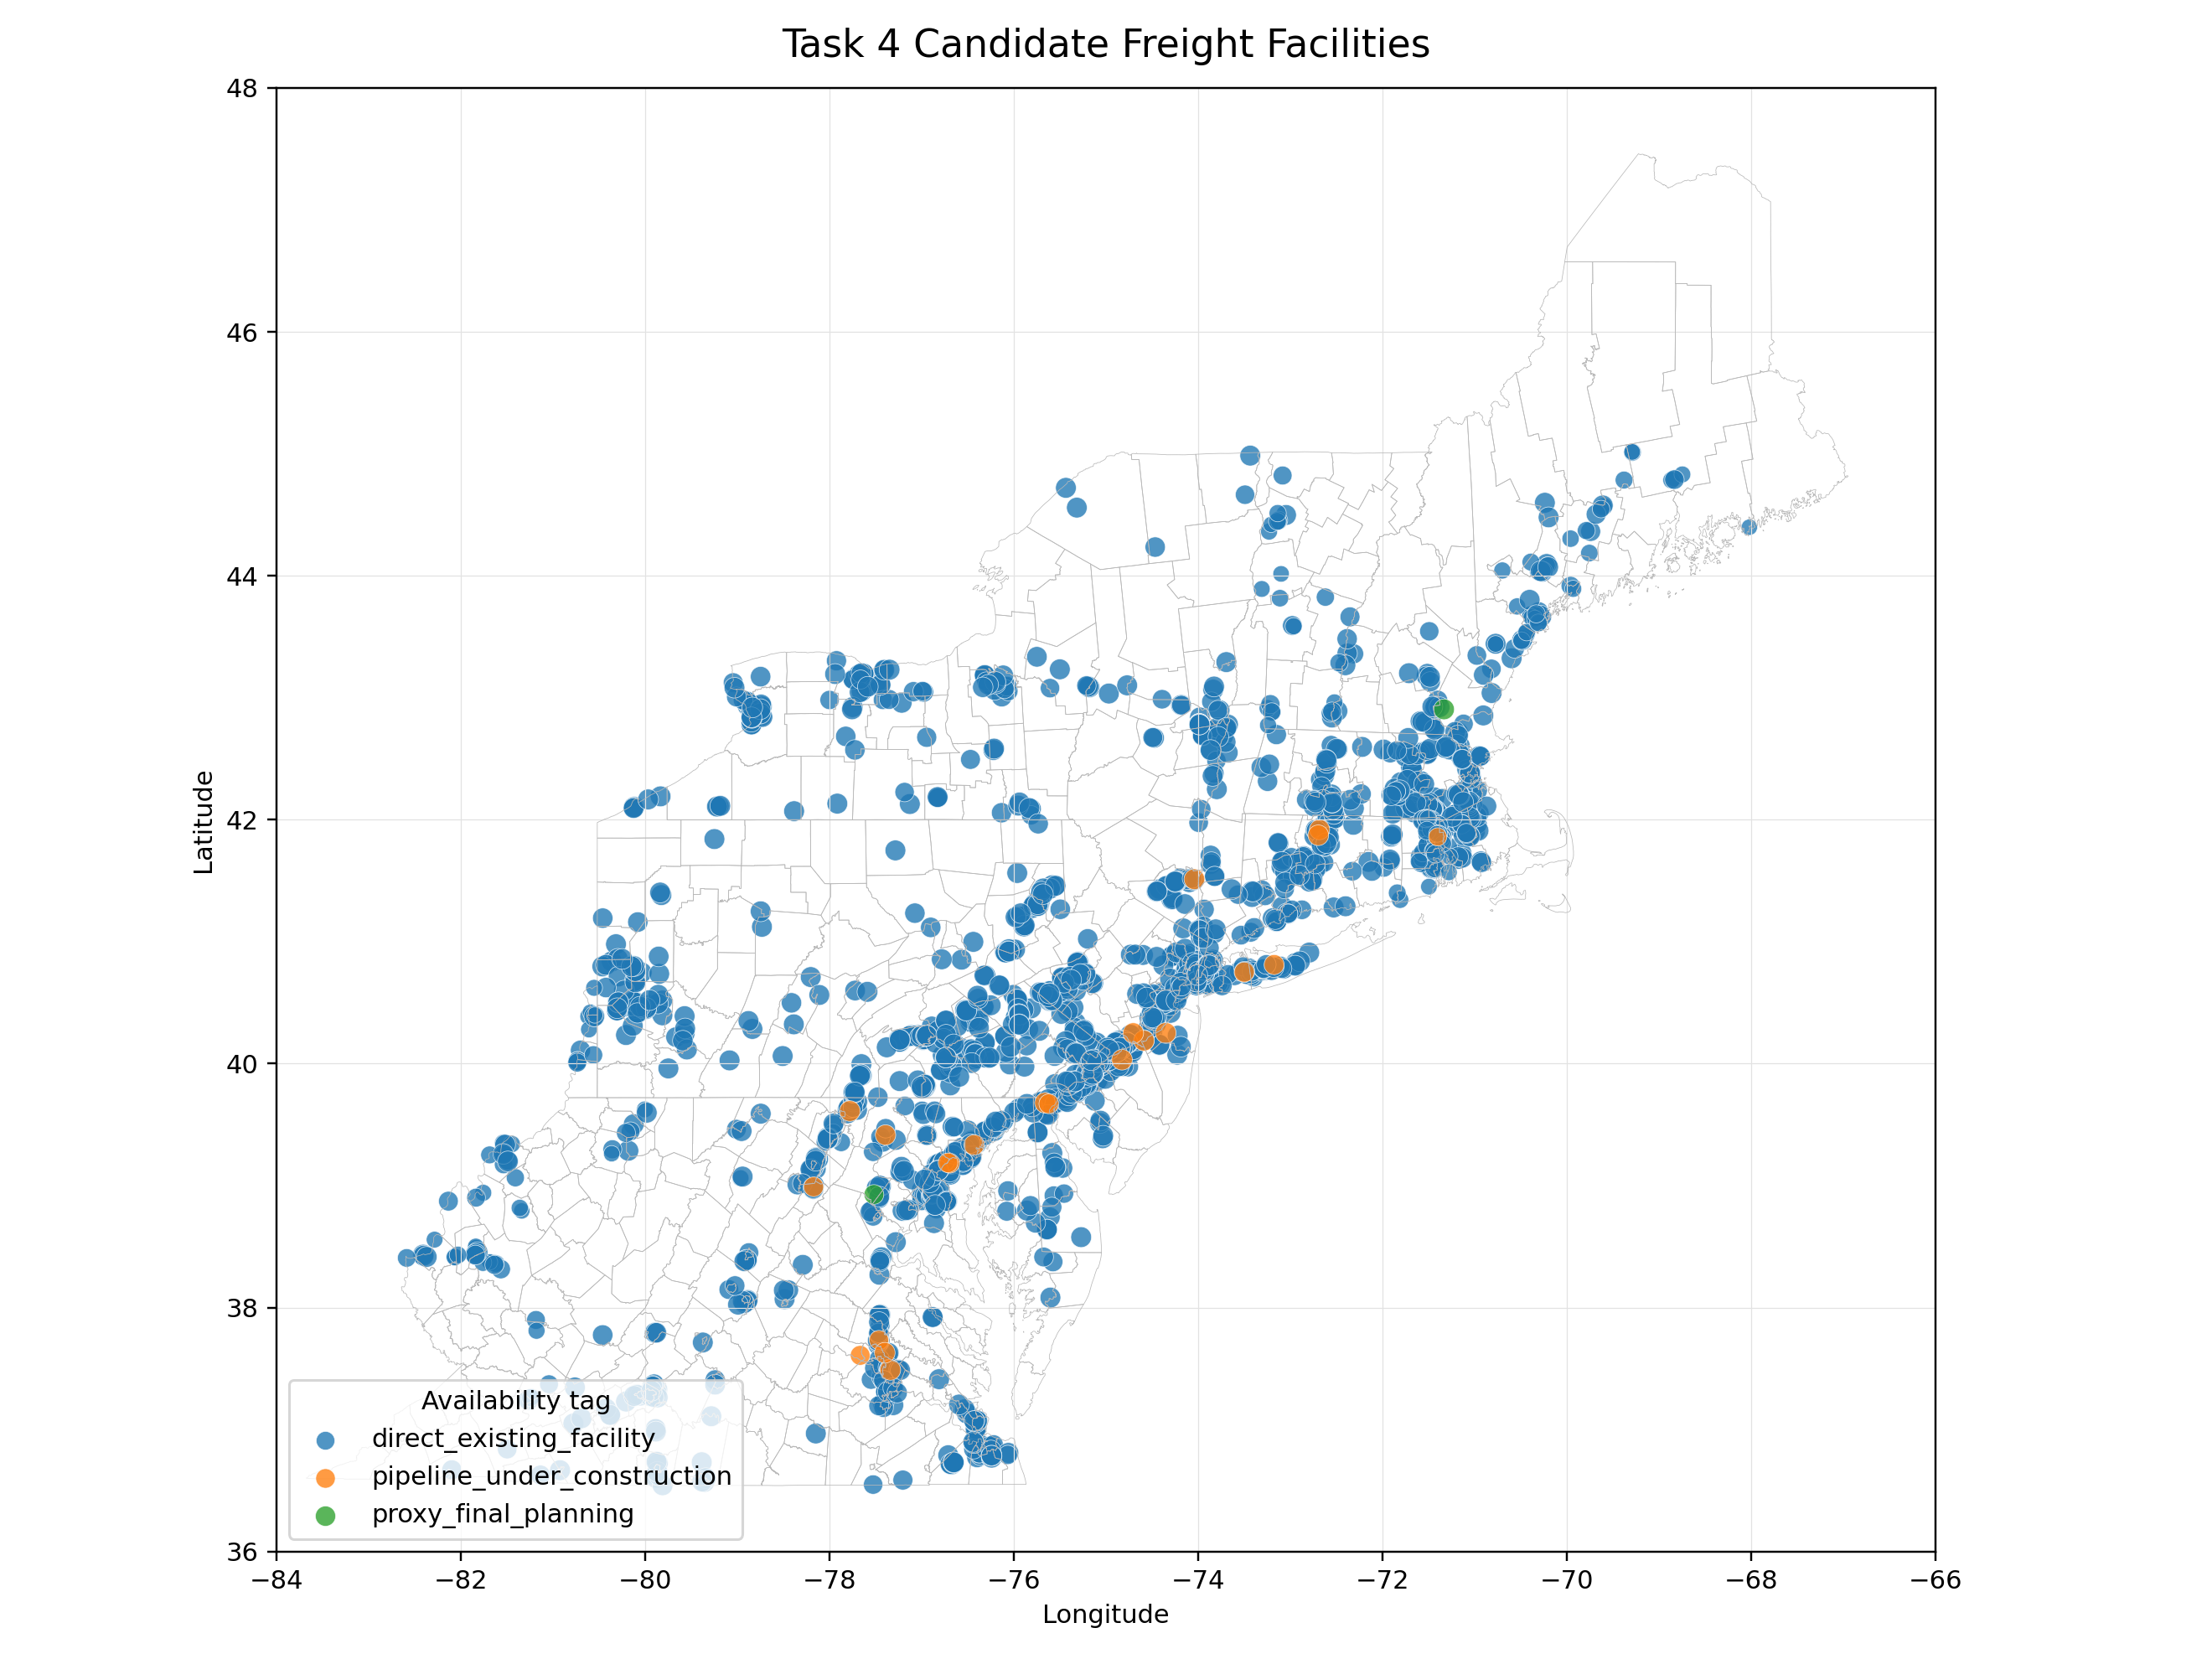
\includegraphics[width=0.92\textwidth]{figures/task4_candidate_map.png}
  \caption{Geographic distribution of 1{,}862 primary regional hub candidates across
    the 14-state Northeast megaregion. Facilities are colour-coded by state. The
    highest-density clusters appear along the I-95 corridor (NJ--PA--MD), the
    Greater Boston belt, and the Virginia--DC logistics spine.}
  \label{fig:task4-map}
\end{figure}

\subsection{Candidate Classification and Downstream Use}

Two output files are produced for Task~5 consumption:

\begin{itemize}
  \item \texttt{primary\_regional\_hub\_candidates.csv} — 1{,}862 facilities satisfying
        all three filters. Each row includes the candidate identifier, state, county FIPS,
        Task~3 region assignment, coordinates, secondary type, building class, building
        status, \texttt{usable\_available\_space\_sf} (the hub capacity parameter $s_h$
        in the Task~5 MIP), and number of loading docks.
  \item \texttt{preprocessed\_capacity\_location.csv} — the full 2{,}064-row pool with
        all computed tag columns. Used as a fallback for regions where the primary pool
        yields insufficient coverage candidates within the 150-mile assignment radius.
\end{itemize}

The \texttt{usable\_available\_space\_sf} field serves directly as the hub capacity
parameter $s_h$ in the Task~5 set-cover formulation. The field represents verified
available square footage rather than total building area, ensuring that hub capacity
assignments reflect what can actually be activated in the near term.
